%% The following is a directive for TeXShop to indicate the main file %!TEX root = ../MJThesis.tex
\acresetall

\chapter{The crystallization and X-ray diffraction of the S-layer protein, RsaA}
\label{ch:crystal}
\begin{epigraph}
  \emph{``Please forgive me for presenting, on such a great occasion, results which are still in the making, but the glaring sunlight of certain knowledge is dull and one feels most exhilarated by the twilight and expectancy of the dawn.''} ---~Max Perutz, 1962 Nobel lecture\\ The father of protein X-ray crystallography.
\end{epigraph}

\section{Introduction} % (fold)
\label{sec:crystal_introduction} 

\Acp{S-layer} are para-crystalline coatings that
surround microbial cells\upcite[.]{beveridge1997v}
 They have various functions, such as adhesion
and immune evasion in pathogenic bacteria\upcite[;]{DallaireDufresne20141, kern2010bsla}
 protection against phage and predation\upcite[;]{koval1991effect, koval1993predation}
 and as a pseudo-membrane in archeae\upcite[.]{Blaurock01101976}
 \acp{S-layer} are composed of either one or a small number of secreted proteins that self assemble
into a contiguous sheet in the extracellular environment. Despite their
unique features, \acp{S-layer} have not enjoyed the intensive structural
investigations that most other protein families have received, in no
small part due to their proclivity to self-assemble into large polymeric
structures that resist crystallization.

The Gram-negative bacterium \ac{caulobacter} possesses an
S-layer comprised of a single 98.6 kDa protein, RsaA\upcite[.]{smit1981periodic}
 This particular S-layer has been pursued as a potent platform for peptide display and
protein expression\upcite[.]{smit2008heads}
RsaA is secreted from the cell via a type 1
secretion system\upcite[.]{walker94}
 RsaA shares little to no sequence similarity to any
other known protein, except for in the conserved \ac{rtx}
motifs canonically found in all type 1 secreted proteins\upcite[.]{chenal2009rtx, bingle2000secretion}
 RsaA further isolates itself in its sequence by featuring a uniquely limited amino
acid composition that is biased towards small, simple residues. This bias
towards `cheaper' amino acids is thought to be an evolutionary strategy
for secreted proteins conserved across micobial life and especially in
\ac{caulobacter}\upcite[.]{smith2010economical}

All crystallographic studies of \ac{S-layer} proteins have to inhibit \ac{S-layer} formation. In the
past co-crystallization with nanobodies\upcite[]{baranova2012sbsb}
 and truncation\upcite[]{Pavkov20081226}
 approaches have resulted in monodisperse, crystallizable proteins. Here we describe the
expression of a 804 \ac{aa} C-terminal fragment of RsaA (RsaA \del 0--222) from
its native host, \ac{caulobacter}. The untagged protein was purified
from culture supernate and crystallized by hanging-drop vapour
diffusion. Crystals were grown that diffracted to 2.0 \AA.
Diffraction data were collected at both the \ac{cls} 
and the \ac{ssrl}. RsaA is the first Gram-negative S-layer protein to be crystallized.

\section{Materials and Methods}
\label{sec:crystal-materials-and-methods}

\subsubsection{Macromolecule Production}
\label{sub:crystal-macromolecule-production}

Our protein construct, RsaA \del 0--222, was expressed in both a traditional
\ac{ecoli} expression system and our lab's \ac{caulobacter}
protein system\upcite[.]{bingle1997expression, UmeloNjaka20011406, Bingle1990143}
 All attempts to produce protein in \ac{ecoli}
resulted in highly insoluble inclusion bodies that resisted
refolding. Expression levels of RsaA in its native host is notably high\upcite[]{lau2010analysis} but
the system did not initially produce protein in an appropriate form.

The reasons for an N-terminal truncation of RsaA are two-fold; deletion
of the N-terminus produces protein that no longer anchors itself to
outer membrane, resulting in soluble supernatant protein; and the
N-terminus has been identified as the center of three-fold symmetry, its
deletion should prevent wide-scale \ac{S-layer} formation and aggregation.

The cells were grown in HIGGM16 medium\upcite[]{smitpilin81}
at 30\cel for 72 hours. 250 \millilitre cultures
were used in 2500 \millilitre wide-bottom fernbach flasks, resulting in shallow
cultures that did not require shaking for sufficient airation as
agitation of the culture led to macroaggregation of the secreted
protein. The cultures were centrifuged at 6300 rpm in JA-10 bottles for
35 min, the supernates were recovered and recentrifuged. The
supernatants were then filtered through a 0.22 \si{\micro\meter} microfilter to ensure
no cells remained. The protein-containing supernatant was initially
concentrated by lyophilization and rehydration to 1/10 the original
volume. The rehydrated protein solution was dialyzed against distillied
water and microfilitered. Purification was performed over a 26/60 S100
Sephadex size-exclusion chromatography column and mobile phase of 200 \si{\milli\molar} \ce{NaCl} and 10 \si{\milli\molar}
Tris pH 7.5. The first major elution peak was pooled and dialyzed
against distilled water and concentrated by placing the dialysis bags on
super-high molecular weight \ac{peg}. The protein
solution was slowly concentrated to a final concentration of 3.5--4
\mgperml.

\subsubsection{Crystallization}\label{crystallization}

Initial sparse-matrix screening was performed using our protein at a
concentration of 9 \mgperml and JGSC Core I, II, III and IV screens. % Cut it out? Ask Murphy lab
 After one week incubation at room temperature, small crystalline shapes were
observed in JGSC Core I well 28 (200 \si{\milli\molar}  \ce{MgCl2}, 100 \si{\milli\molar} Tris pH 7, 20\% \ac{peg}
8000). These crystals were not reproducible in hanging drop vapor
diffusion wells. Very thin plates readily formed once the concentration
of the protein and the \ac{peg} 8000 were both reduced. Improved crystals
formed when \ce{MgCl2} was replaced with \ce{CaCl2}, \ce{SrCl2}, or \ce{BaCl2}; \ce{SrCl2} was
deemed the most succesful at producing crystals. Final crystallization
conditions were 8.5\% \ac{peg} 8000, 100 \si{\milli\molar} Tris pH 7.4, and 150 \si{\milli\molar} \ce{SrCl2}.
Two crystals forms were observed, planar `plate' crystals and hexegonal
columnar crystals. 25\% glycerol was used as a cryo-protectant for all
crystals prior to flash freezing in liquid nitrogen.

\begin{figure}[htb]
  	\begin{center}
   		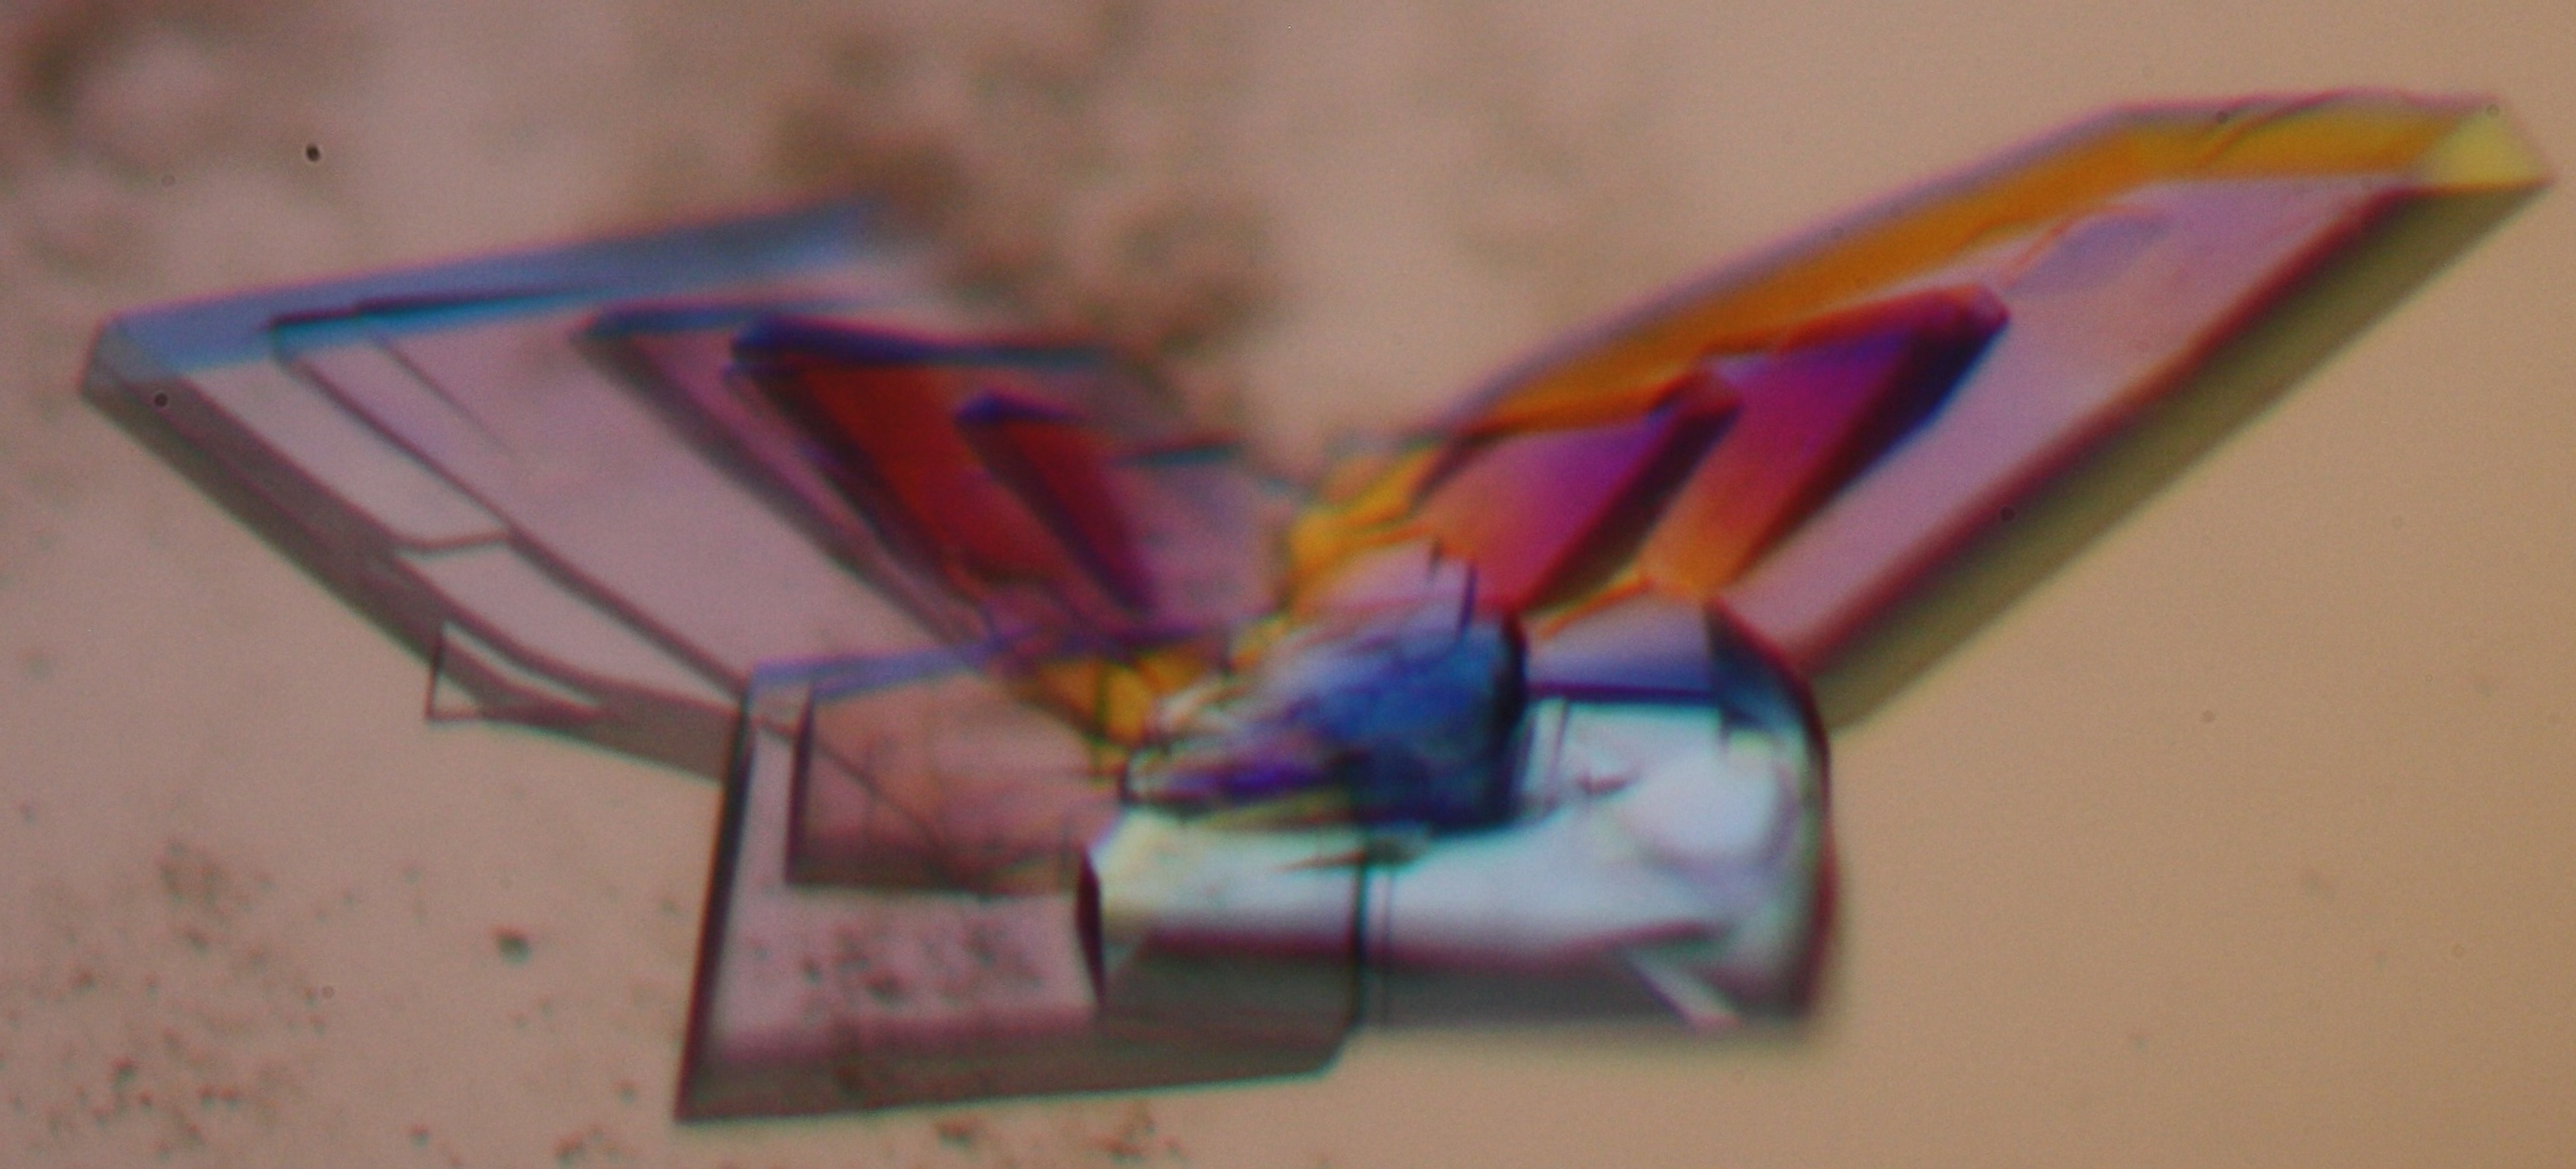
\includegraphics[width=0.7\textwidth]{crystal_chapter/img/bigflowerxtal.jpg}
   	\end{center}
   	\caption[Example of a large cluster of `plate' RsaA \del 0--222 crystals]{An example of a large cluster of `plate' crystals of RsaA \del 0--222. The cluster was just over one millimeter in width from tip to tip. The largest crystal, on the right, was broken off and diffracted using synchotron radiation, resulting in disappointing resolution. The color is imparted by a polarizing filter on the microscope, the crystals are naturally colourless.}
   	\label{fig:crystal-flower}
\end{figure}
\begin{figure}[htb]
  	\begin{center}
   		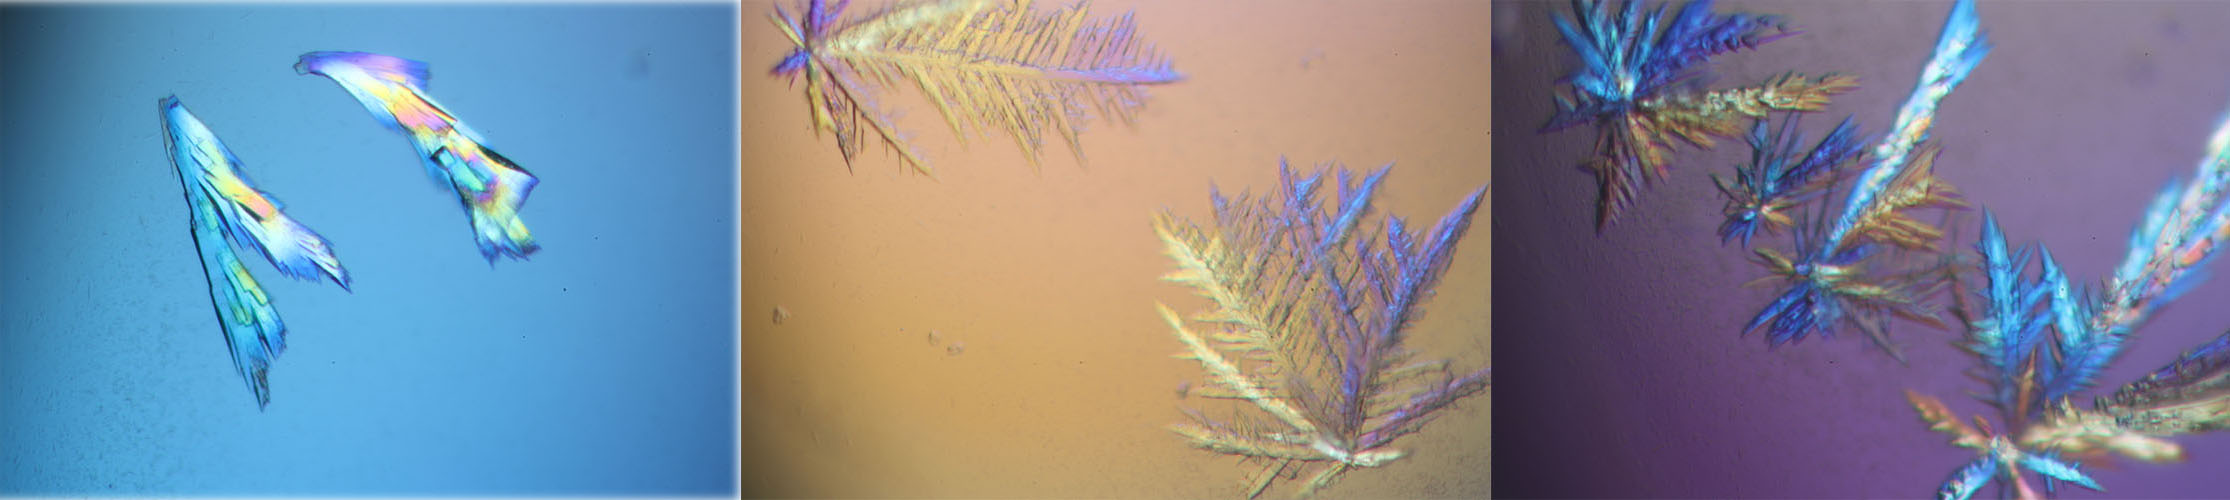
\includegraphics[width=0.9\textwidth]{crystal_chapter/img/dendroXtals.jpg}
   	\end{center}
   	\caption[Example of a `dendritic' RsaA \del 0--222 GSSC723 crystals]{The examples of `dendritic' crystals formed when the RsaA \del 0--222 GSSC723 protein construct was crystallized. The color is imparted by a polarizing filter on the microscope, the crystals are naturally colourless.}
   	\label{fig:crystal-flower}
\end{figure}